\documentclass[../report.tex]{subfiles}
\begin{document}

\graphicspath{{img/}{../img/}}

\section{Product Breakdown}

Et Product Breakdown Diagram laves ved at se p� et helt projekt og finde ud af hvilke dele det best�r af. Man inddeler alts� projektet i produkter som n�r de bliver sat sammen vil udg�re et f�rdigt projekt. Hvert produkt kan s� deles ind i mindre produkter, ligesom man g�r med hele projektet\cite[p.~59-61]{hughescotterell09}. Produkterne vil p� den m�de danne et hierarki hvor det �verste produkt vil v�re hele projektet og de nederste produkter vil v�re detaljerede produkter som er mere h�ndgribelige.

Ved at lave et Product Breakdown Diagram f�r man et bedre overblik over, hvad der skal laves for at projektet bliver f�rdigt. Senere i projektet kan man ogs� bruge det til at holde styr p� om alle dele af projektet er blevet lavet.

I target-projektet blev der lavet et Product Breakdown Diagram med relativt f� produkter (se figur \ref{fig:Product Breakdown Diagram}). Det er med andre ord ikke blevet brudt ned i meget detaljerede produkter. Selve Product Breakdown Diagrammet blev prim�rt brugt i starten af projektet, til at f� et overblik hvad der skulle laves, Men det blev ogs� brugt som basis for at lave et Activity Breakdown Diagram. 


\begin{figure}[H]
\hspace{-2.6cm}
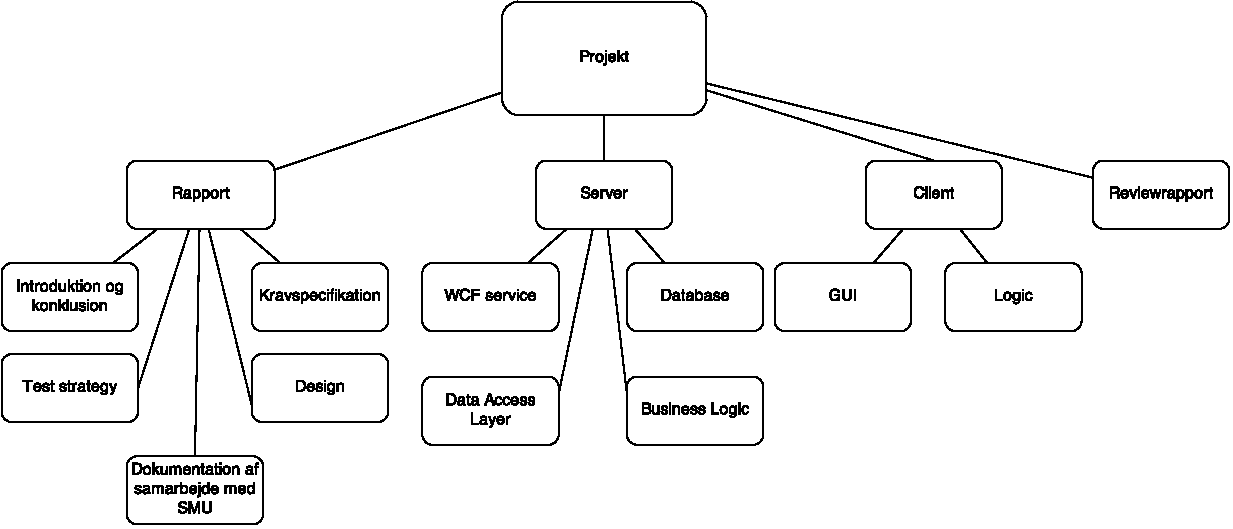
\includegraphics[ scale=0.9]{ProductBreakdownDiagram.pdf}
\caption{Product Breakdown Diagram fra target-projektet}
\label{fig:Product Breakdown Diagram}
\end{figure}



\end{document}